The benefits of C integration are numerous: The major computer operating systems are written in C,(cite) the C runtime is ubiquitous and generally doesn't conflict with other language runtimes, and C is conducive to high performance programming.

Language designers and maintainers commonly provide support and documentation for how to integrate C modules into projects based in their languages.  Of the top ten most popular languages by pull request on Github\cite{Octoverse}, nine have native support for calling C code\cite{JavascriptCiface}\cite{PythonCiface}\cite{JavaCiface}\cite{RubyCiface}\cite{PHPCiface}\cite{DotNetCiface}\cite{GoCiface}(cite C++) (the exception, CSS; C, in tenth place, obviously links with itself).

\begin{figure}[htbp!]
        \centering
        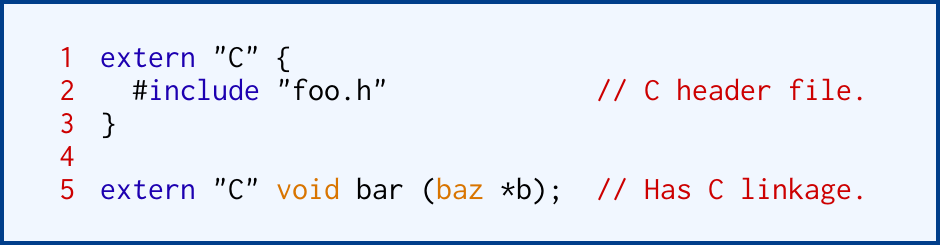
\includegraphics[scale=0.25]{gfx/extern}
        \caption{Example of C++ importing code from and exporting code to C.}
        \label{fig:extern-example}
\end{figure}

As in Fig.~\ref{fig:extern-example}, C++ goes to lengths to be compatible with C in both directions.  By using \texttt{extern \textquotedbl{}C\textquotedbl{}}, a symbol can be declared with C linkage, and since all of the native C types correspond to native types in C++, calling back-and-forth between languages is easy.

